\documentclass[]{article}

\usepackage[utf8]{inputenc}   % pro unicode UTF-8
\usepackage[czech]{babel}
\usepackage{hyperref}
\usepackage{float}
\usepackage{caption}
\usepackage{graphicx}
\usepackage{amsmath}
\usepackage{pdfpages}
\usepackage{fancyhdr}
\usepackage{matlab-prettifier}
\usepackage{xspace}
\usepackage{multicol}
\usepackage{longtable}
\usepackage{amssymb}
\usepackage{wrapfig}
\usepackage{caption}
\usepackage{subcaption}
\usepackage{acro}
\usepackage{translations}
\usepackage{matlab-prettifier}
\usepackage[left = 3cm,right = 3cm,top=3cm,bottom = 3cm]{geometry}
\usepackage[bottom]{footmisc} % poznámky pod čarou se zarovnají automaticky naspod stránky
\usepackage{pdfpages} % podpora vložení stran z pdf
\usepackage{pdflscape} % podpora otočení stránky

%%%%%%%%%%%%%%%%%%%%%%%%%%%%%%%%%%%%%%%%%%%%%%%%

\setboolean{@twoside}{false}
\pagestyle{fancy}
\fancyhead{}
\fancyhead[L]{LaTex vzor pro osobní dokumenty na FELu}

\fancyfoot{} % clear all footer fields
\fancyfoot[L]{Tomáš Dudáček}
\fancyfoot[C]{\thepage}
\fancyfoot[R]{\today}

%%%%%%%%%%%%%%%%%%%%%%%%%%%%%%%%%%%%%%%%%%%%%%%%

\DeclareAcronym{MEMS}{
    short=MEMS,
    long=Micro Electro Mechanical Systems
}


%%%%%%%%%%%%%%%%%%%%%%%%%%%%%%%%%%%%%%%%%%%%%%%%

\renewcommand{\figurename}{Obrázek}
\renewcommand{\tablename}{Tabulka}
%\newcommand{\MATLAB}{\textsc{Matlab}\xspace}

\newcommand{\mycomment}[1]{}

%%%%%%%%%%%%%%%%%%%%%%%%%%%%%%%%%%%%%%%%%%%%%%%%

\author{Tomáš Dudáček}

%%%%%%%%%%%%%%%%%%%%%%%%%%%%%%%%%%%%%%%%%%%%%%%%

\begin{document}

\begin{titlepage}
    \begin{center}
        \vspace*{1cm}
 
        \textbf{Osobní LaTex vzor pro dokumenty na ČVUT FEL}
        \vspace{1.5cm}
 
        \textbf{Tomáš Dudáček} 
        
 
        \vfill
             
        \vspace{0.8cm}
      
        
\includegraphics[width=0.4\textwidth]{foto/logoFEL.jpg}  
    \end{center}
 \end{titlepage}


%%%%%%%%%%%%%%%%%%%%%%%%%%%%%%%%%%%%%%%%%%%%%%%%

\tableofcontents

\pagebreak
\printacronyms[name=Zkratky]


\pagebreak

\section{Kapitola}
\subsection{Podkapitola}

Citace \href{https://www.overleaf.com/learn/latex/Bibliography_management_with_bibtex}{https://www.overleaf.com/learn/latex/Bibliography\_management\_with\_bibtex} 
\cite{PetitSieffermann2007}. \\
Tabulky \href{https://calc2latex.sourceforge.net/}{https://calc2latex.sourceforge.net/} \\

\begin{table}[H]
\centering
    \caption{\label{tab:table_dists} Účinný dosah ultrazvukových rušiček pro různá zařízení}
    \begin{tabular}{ |c|c| } 
     \hline
     Použité nahrávací zařízení & Maximální efektivní dosah rušení $[m]$ \\
     \hline
     iPhone 5s & 2,5 \\ 
     iPhone 7  & 3 \\ 
     Xiaomi Redmi 5 & 2,3 \\ 
     Samsung Galaxy A5 & 2 \\ 
     Honor 7X & 2,2 \\ 
     Sony Ericsson TM506 & 1 \\ 
     HP 250 G6 (laptop) & 2 \\ 
     \hline
    \end{tabular}
\end{table}

Obrázky :

\begin{figure}[H]
\centering
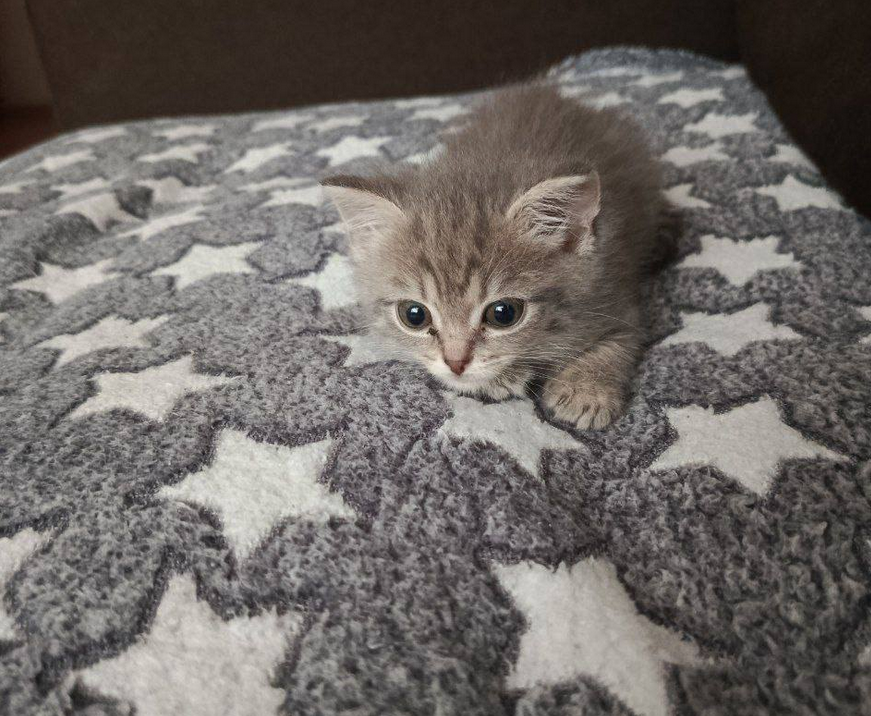
\includegraphics[width=0.7\textwidth]{foto/ScreenshotIllegallySmolCats.png}
\caption{\label{fig:cato} \cite{cato}}
\end{figure}

\begin{figure}[H]
\centering
    \begin{subfigure}[b]{0.49\textwidth}
        \centering
        \raisebox{0.165\textheight}{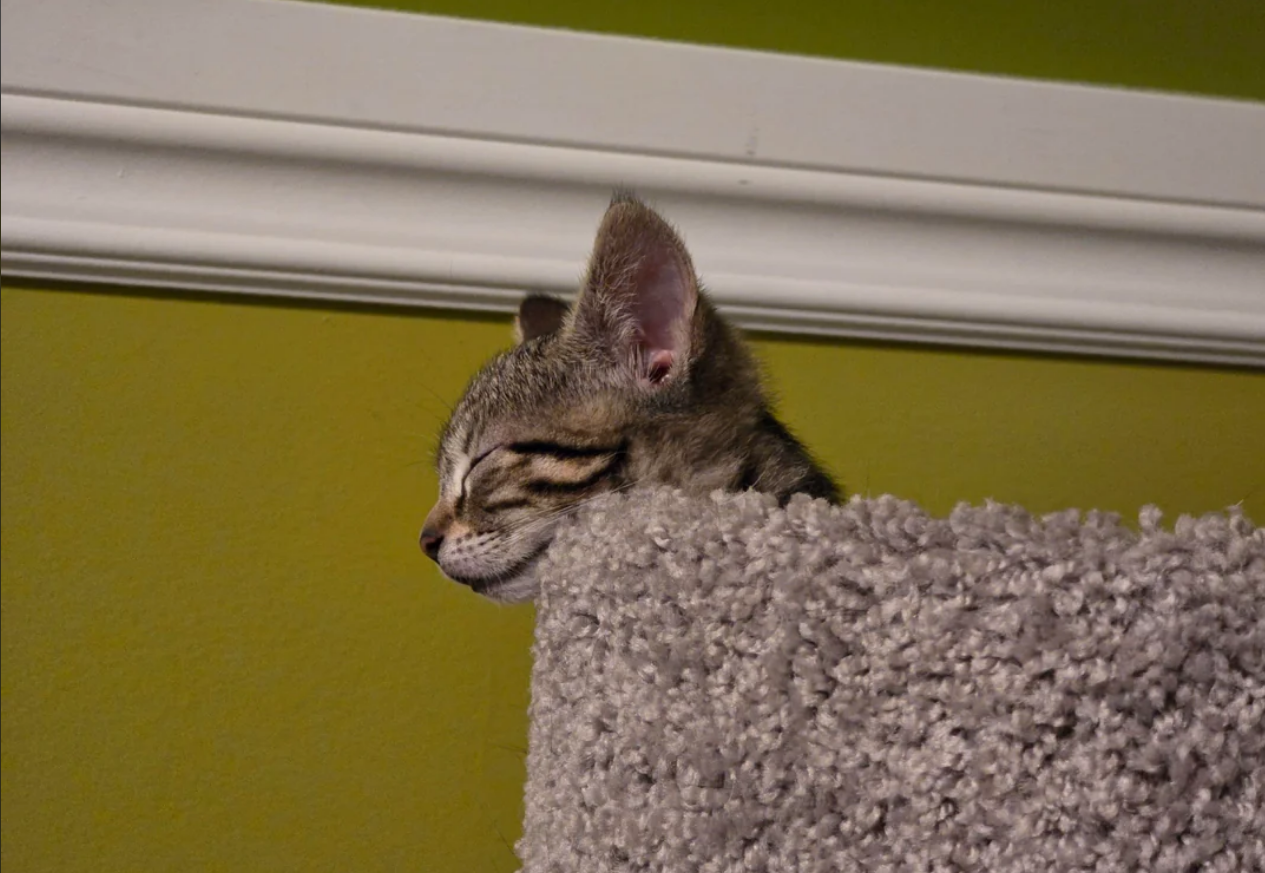
\includegraphics[width=0.9\textwidth]{foto/ScreenshotIllegallySmolCats2.png}}
        \caption{\label{fig:cato2} \cite{cato2}}
    \end{subfigure}
    \hfill
    \begin{subfigure}[b]{0.49\textwidth}
        \centering
        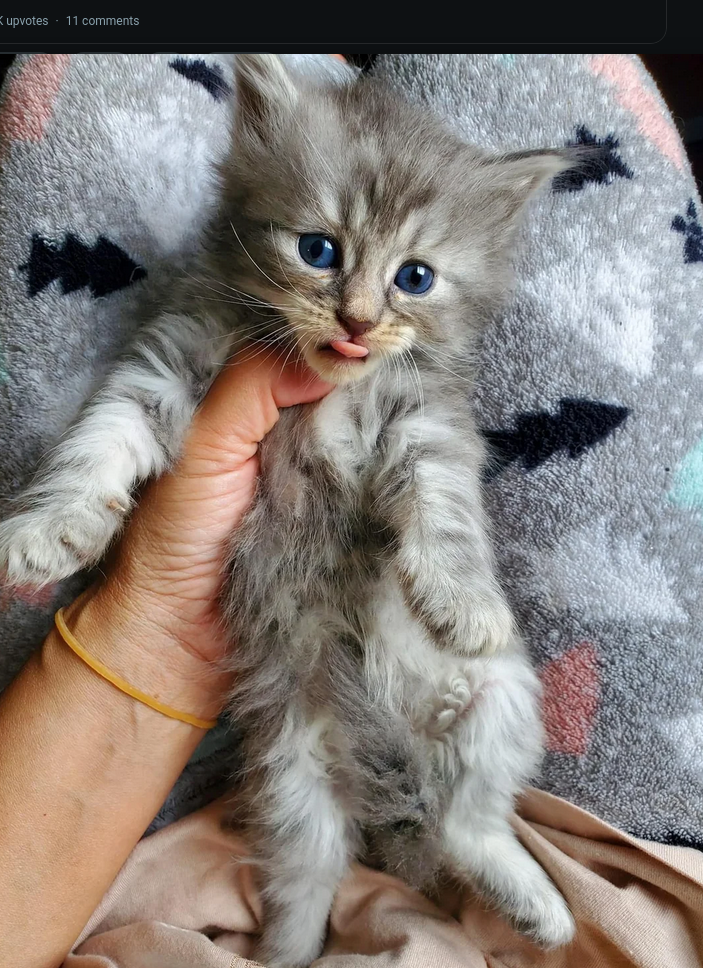
\includegraphics[width=\textwidth]{foto/ScreenshotIllegallySmolCats3.png}
        \caption{\label{fig:cato3} \cite{cato3}}
    \end{subfigure}

    \caption{\label{fig:catos} Kočky vedle sebe}
\end{figure}

Zkratky: Poprvé dlouze - \ac{MEMS} podruhé krátce - \ac{MEMS}

Rovnice (číslované):

\begin{equation}
    S_{out} = A_1 S
\end{equation}

Reference: Obrázek \ref{fig:cato}

\pagebreak
\section{Zdroje}
\begingroup
\renewcommand{\section}[2]{}
\bibliographystyle{ieeetr}
\bibliography{references} 
\endgroup

\end{document}

